\documentclass{article}
\usepackage{tikz}
\title{Illustrasjon av PCB-layout}
\begin{document}
\maketitle

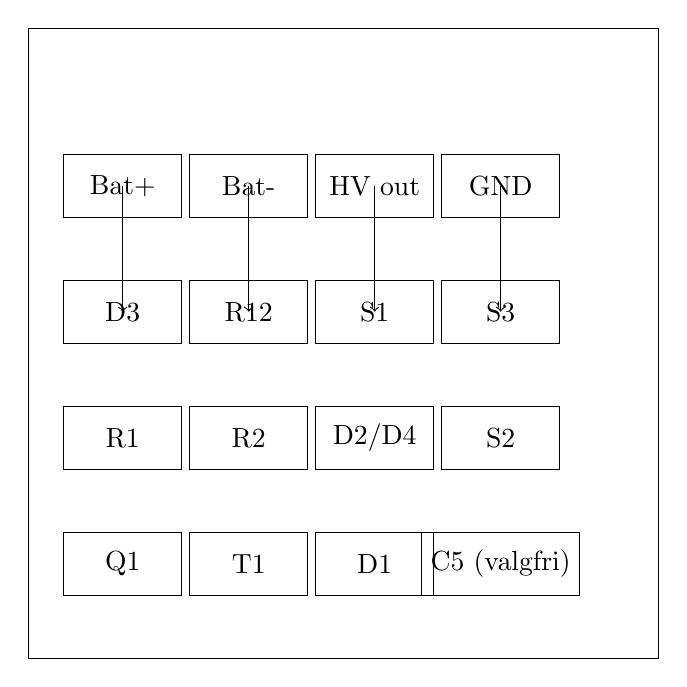
\begin{tikzpicture}[scale=0.4, every node/.style={draw, minimum width=1.5cm, minimum height=0.8cm, align=center}]
% PCB outline
\draw (0,0) rectangle (20,20);
% Komponenter
\node at (3,3) {Q1};
\node at (7,3) {T1};
\node at (11,3) {D1};
\node at (15,3) {C5 (valgfri)};
\node at (3,7) {R1};
\node at (7,7) {R2};
\node at (11,7) {D2/D4};
\node at (15,7) {S2};
\node at (3,11) {D3};
\node at (7,11) {R12};
\node at (11,11) {S1};
\node at (15,11) {S3};
\node at (3,15) {Bat+};
\node at (7,15) {Bat-};
\node at (11,15) {HV out};
\node at (15,15) {GND};
% Tilkoblinger (forenklet)
\draw[->] (3,15) -- (3,11);
\draw[->] (7,15) -- (7,11);
\draw[->] (11,15) -- (11,11);
\draw[->] (15,15) -- (15,11);
\end{tikzpicture}

\textbf{Merk:} Dette er kun en prinsippskisse. Det endelige PCB-designet må lages i et EDA-verktøy.
\end{document}
